\chapter{Literature Survey}

\section{The PUF concept}
The simplest sentence to describe PUF is "A PUF is an object's fingerprint" \cite{Reference4}. The fingerprint can represent a specific human in the world, such as the PUF can represent
an object. The fingerprint is inherently created when people was born, and the so does PUF, which is inherently exist in an object according to unique manufacturing random variation \cite{Reference4}.
With the representation and inherent property, the fingerprint and the PUF is said to be unclonable since it is impossible to control and predict human's fingerprint. This is an important concept for PUF. \par

This intrinsic property can be extract from chip which has PUF circuit existed inside \cite{Reference2}. The way PUF works is by entering a certain length of bits(so called challenge) into the PUF, and it will
generate another specific length of bits(so called response). According to the property of PUF that was discuss above, it is impossible to find two different PUF that will produce the same response when entering same challenge(See Figure \ref{fig:figure1}).
\begin{figure}[ht]
\centering
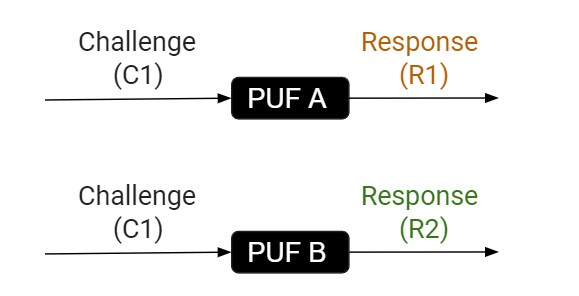
\includegraphics[width=8cm]{figures/figure1.jpg}
\caption{Different PUF that generate different response when input same challenge}
\label{fig:figure1}
\end{figure}

\section{Weak and strong PUF}
PUF can be classified into two categories, weak and strong PUF according to the strength of PUF. The strength of PUF indicate the number of challenge response pairs(so called CRPs) can be generate 
from the PUF \cite{Reference1}. The higher numbers of the CRPs can a PUF generate, the better strength it has. For the weak PUF, it represent the PUF that has smaller set of CRPs. While it is impossible to 
create a clone of PUF, but with small set of CRPs, this will allow attacker to have physical access to all the CRPs \cite{Reference1}. With the knowledge of CRPs, attacker can easily response the corresponding
response to challenge as like they have a clone(See Figure \ref{fig:figure2}). The weak PUF can be use for authentication and key storage. However, since weak PUF's CRPs can be fully access, ensuring having a secure environment and whether the original PUF is being evaluating is relatively important \cite{Reference1}.
\begin{figure}[ht]
    \centering
    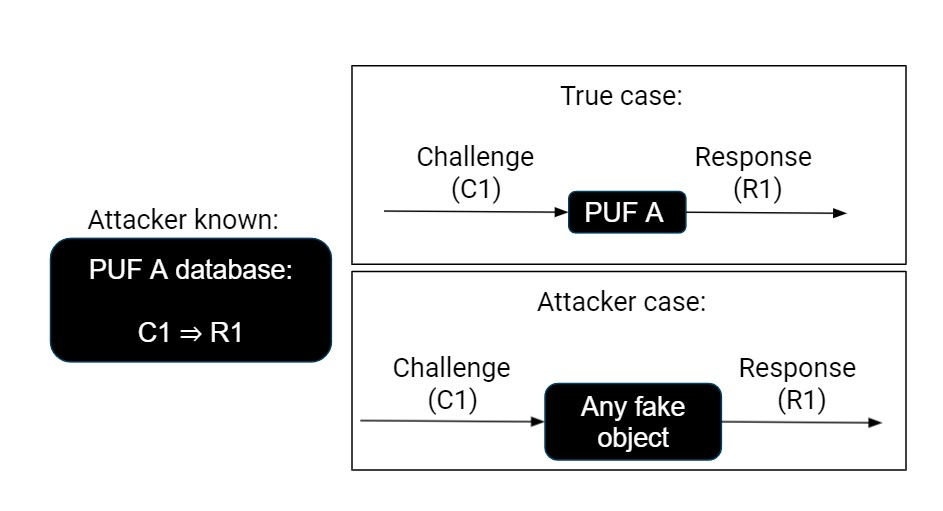
\includegraphics[width=9cm]{figures/figure2.jpg}
    \caption{Attacker can perform same behavior as Weak PUF when have fully access to CRPs}
    \label{fig:figure2}
    \end{figure}

For strong PUF, means the number of CRPs is significantly large that even attacker get access, having throughout knowledge of CRPs is impossible. While the number of CRPs is so large,
and the CRP are randomly selected in usage, the probability that attacker has knowledge about the CRP currently using is small. In addition, each CRPs that is used once will 
be discarded(See Figure \ref{fig:figure3}) so even if attacker recorded certain CRPs, they will not be able to put into use. The strong PUF can also be use for authentication but do not need to protect CRPs
as serious as weak PUF.

\begin{figure}[ht]
    \centering
    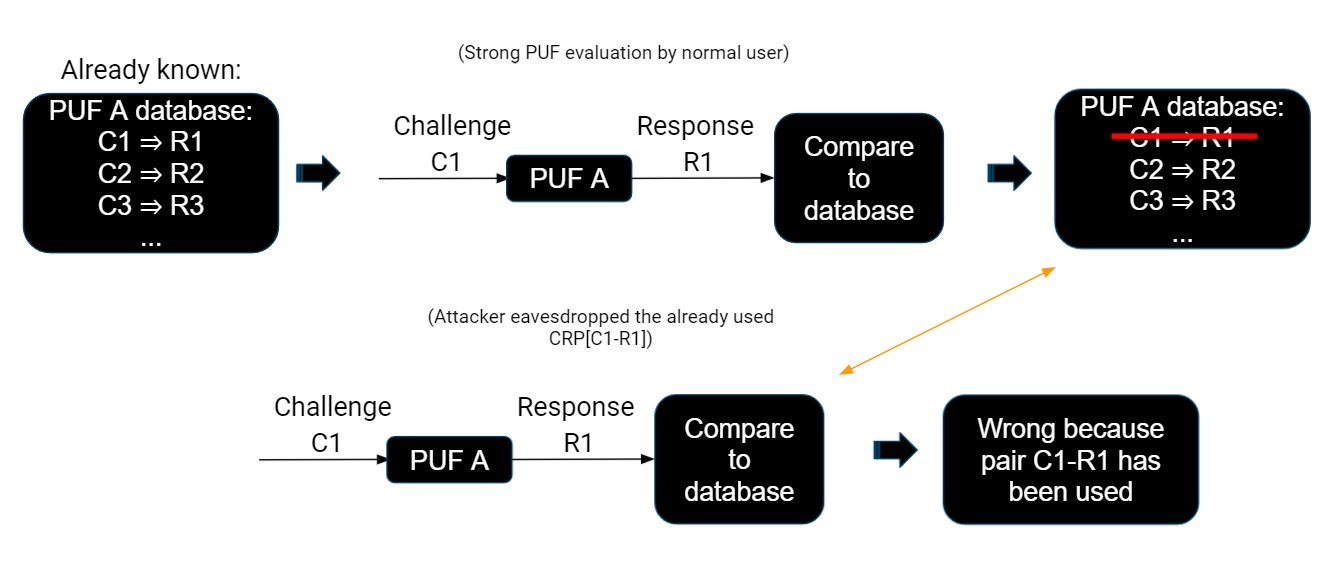
\includegraphics[width=15cm]{figures/figure3.jpg}
    \caption{Different PUF that generate different response when input same challenge}
    \label{fig:figure3}
    \end{figure}

\section{Introduce to weak and strong then authentication stage or ...}

\section{Summary}


